\part{Analysis}

A hand digit recognition neural network (HDR-NN) model is implementated in \texttt{C}, \texttt{C++}, Eigen, Python Numpy and Pytorch. The performance of HDR-NN training implementations was evaluated on the iMX6SDB evaluation board, which was programmed with an Embedded Linux built using The Yocto Project. To gauge the effectiveness of the models, we compared model accuracy, execution time, and peak memory usage while altering the number of layers and neurons in each layer. The results of these measurements are presented in the following chapters along with discussions on the obstacles encountered in developing the NN model and compiling it to operate on the target hardware.

\subsection*{An Overview}

A hand digit recognition neural network is implemented in different paradigms, specifically \texttt{C}, \texttt{C++}, Python, and Pytorch, which are the benchmark applications. Each of thess applications contain a fully connected feedforward neural network composed of multiple layers of neurons connected in a directed graph. The model has a constant input size of 784 which correspond to the 28 x 28 pixel dimensions of the images of the MNIST dataset. The output size of the network is 10, corresponding to the 10 possible digits that the image contains. The number and size of the hidden layers are configurable in each of the different implementations.

The MNIST dataset was selected to train the model, which contains 60,000 training images and 10,000 test images of hand-written digits. The model is trained using stochastic gradient descent, which is an optimization algorithm used to minimize a loss function. The backpropagation algorithm is used to calculate the gradients of the loss function with respect to the weights of the network. Finally, the mean square error loss function is used to measure the difference between the predicted output and the actual output of the network. The values of the biases and weights are initialized randomly with the PNGR random generator and a starting seed which are chosen to be identical for the different benchmark applications. The training hyperparameters are set to 30 epochs with a batch size of 10, a learning rate of 3, with the network using the sigmoid activation function.

It is essential that the hardware utilsed for benchmarking closely resembles the Scania ECU's IMX6 processor, as this will make it easier to replicate the experiment on a repurposed ECU and will also provide the most precise results. The IMX6Q-SABRE Smart Devices evaluation board, which is armed with four 32-bit Cortex A9 cores, is an ideal choice. The Cortex A9 core is equipped with ARM V7 instruction set architecture and a powerful VFPv3 floating point unit with NEON SIMD capabilities. The processor has 32 KB instruction and data L1 caches, 1 MB L2 cache and 1 GB DDR3 SDRAM memory. The benchmark applications are designed to be run on a single core of the IMX6 processor, although it supports quad-core, to ensure the experiment is straightforward and easier to manage. This will also guarantee that the results are precise and accurate.

The yocto project is used to create a custom embedded linux distribution for the \texttt{imx6qsabresd} machine. The NXP yocto project guide (link) provides the instructions for building the Linux image, and additional packages such as cmake, python3 are installed during the build. The resulting image file, which used to flash the hardware, has a size of ~300Mb.

The accuracy of the model is evaluated after each training epoch on the MNIST test set. After the training of the model for 30 epochs, the final weights and biases of the network and the accuracy on the test set are saved for analysis. This data is used to verify the correctness of the NN model in each benchmark application.

The GNU time program is a great tool for monitoring the performance of applications. It allows us to measure the execution time and peak memory usage, which is used to compare the effectiveness of training the neural network model on the custom hardware implemented with different paradigms.

A python script was developed to run the experiment, executing each of the benchmark applications (\texttt{C}, \texttt{C++},, Python, Pytorch) one after the other. Every benchmark application is designed to be repeated 10 times, and all the measurements for each of the hidden layer configurations are saved for each of these iterations. The average values of the model accuracy, execution time and peak memory usage across all iterations are utilized for the analysis.

% ============================================
%        Measurement
% ============================================

\chapter{Measurement}

The benchmark applications were executed on an embedded linux operating system and the measurements were taken primarily based on the \textit{times} system call and perf\_events linux API. The primary tools for current measurement values given in the following chapter were taken using the GNU time. GNU Time provides timing statistics such as the elapsed real time between invocation and termination, the user CPU time, and the system CPU time, the later two via the \textit{times} system call API. GNU Time also provides output lots of useful information on other resources like memory, I/O and IPC calls where available.

The priliminary measurements for the different executions completed with different learning algorithm parameters and model shapes across implementations were timing statistics and maximum resident set size (alternatively refered to as peak memory utilisation in the following chapter)

\section{Benchmark Application Parameters}

The benchmark applications all had the same configurable parameters for their learning algorithm and network structure. Initial testing of the different benchmark applications were completed seperately with different configurations. These test runs were used to come up with estimates as to how long each run of the training sequence with the different parameters would take and then used to come up with the network shape sizes, and other learning algorithm parameters.

Initially, the network's single hidden layer shape was varied according to powers of two, with the \texttt{C} and \texttt{C++} variants tested with 2, 4, 8, 32, 128, 256, 512, 1024 and so on before adding another hidden layer. The additional hidden layer varied sizes from (16, 16), to (32, 16) and (16, 32), then (128, 16), etc.

% ============================================
%        Results
% ============================================

\chapter{Results}

This chapter presents the results of the project. The first section contains a brief look at the analysis on application correctness and the neural network accuracy. The second section considers the performance of the benchmark applications followed by the third section that details their differences. The fourth and concluding section describes the efforts in repurposing the Scania ECUs.

% \section{Coefficient of variation}
% A total of 10 iterations were conducted to ensure that the results remained consistent. To assess the degree of variability among the various trials, the mean and standard deviation were calculated across all runs, and their ratio was determined. This ratio indicates the level of variation between the different tests.

% TODO: we also reason the impact of execution time in the decision to skip some network configurations and add a table of the experiments conducted

\section{Evaluating Correctness}

% \subsection{Accuracy}

As the benchmark applications are developed to be identical by keeping the same structure and configurations, the model accuracy is expected to be similar. The (figure 6.1) showcases that the different implementations perform similarly irrespective of the number of parameters.

\begin{figure}[!ht]
	\centering
	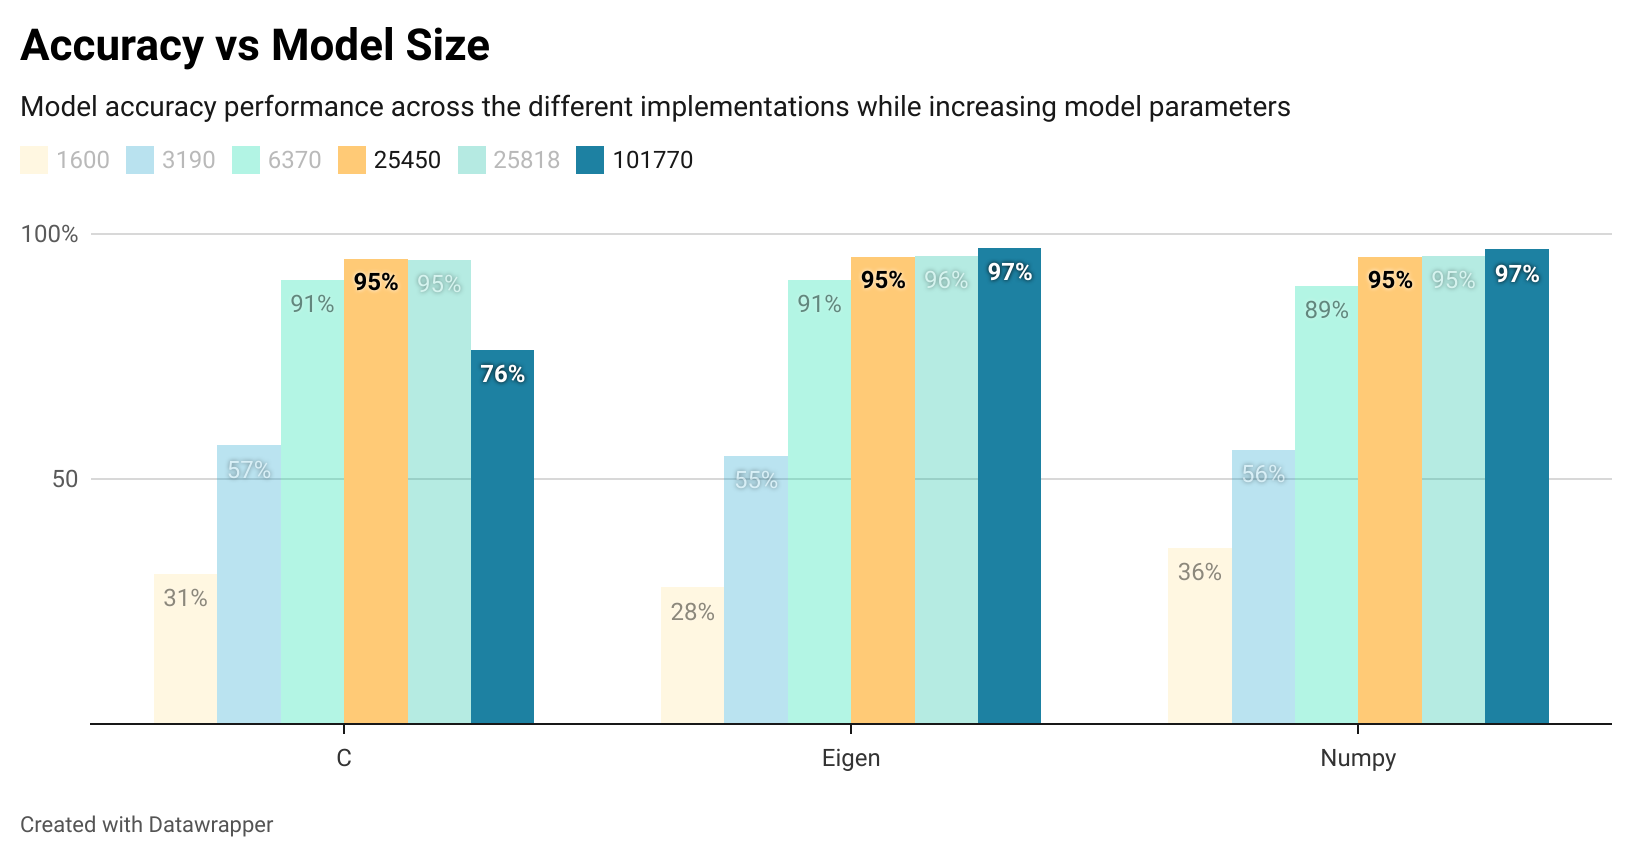
\includegraphics[scale=0.32]{accuracy}
	\caption[HDR-NN Accuracy]{Comparing the accuracy of the different HDR-NN implementations.}
\end{figure}

Further, an abnormal behaviour can be observed when the number of parameters exceeds 101770. The accuracy of the \texttt{C} implementation decreases due to (an unknown bug).

% To improve accuracy, adding another layer with 16 neurons is found to be beneficial without significantly increasing the time required for computation. In fact, for larger network sizes, it is observed to even reduce the computation time required. (separate plot for this behaviour)

% TODO: evaluate the mean squared error in accuray between the benchmark applications

% \subsection{Weights and Biases}

% (TODO: evaluate the mean squared error in the generated weights and biases between the different implementation. Also, reason how the data structure in each of the implementation influence the error.)

\section{Evaluating effectiveness}

% TODO: Something should go here format wise

The primary measures used to evaluate the program performance was execution time and memory utlisation while the applications completed their neural network training.

\subsection{Execution Time}
The training time of the neural network applications increases exponentially as the network size increases by the power of 2 because the number of parameters in a fully connected network increases exponentially as the number of neurons increases. This leads to an increase in the amount of calculations needed for the network to learn, resulting in a longer run time for the training process. This behaviour can be observeed in (figure 6.2) where the execution time increases drastically as number of parameters increases.

\begin{figure}[!ht]
	\centering
	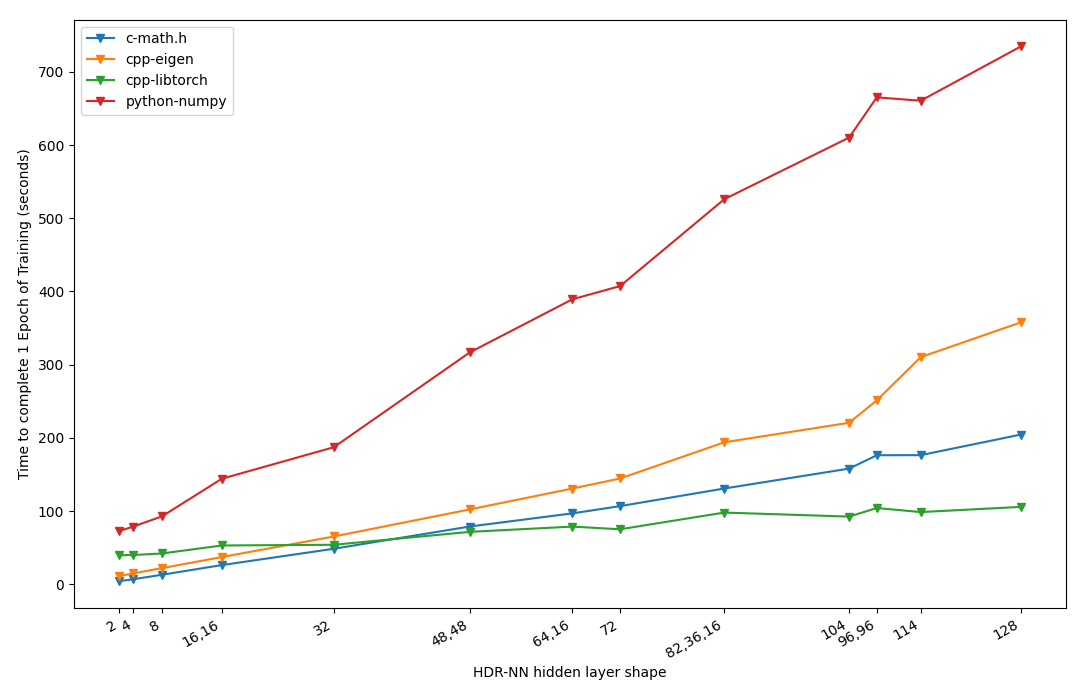
\includegraphics[scale=0.27]{exec-time}
	\caption[Execution Time vs Model Parameters]{Comparing total run time for training the different HDR-NN programs}
\end{figure}

\subsection{Peak Memory Usage}
Regardless of the hidden layer sizes, the peak memory utilisation remains constant for the NN application across all implementations. The \texttt{C++}, Eigen implementation has the lowest run time memory footprint, while Python Numpy is the least efficient.

\begin{figure}[!ht]
	\centering
	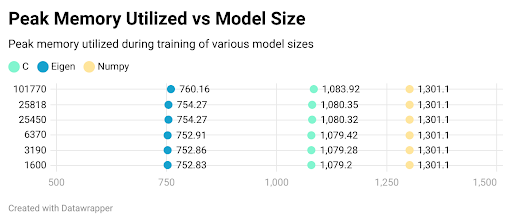
\includegraphics[scale=0.32]{memory-bar}
	\caption[Peak Memory Utilisation]{Peak Memory Utilized during training with different model sizes remain similar within the same implementation}
\end{figure}

% TODO: here we evaluate the percentage/ratio/cov between the applications.

Note that the device RAM is 1024 MB however the peak memory utilisation for both \texttt{C} and Numpy are higher than this value. This can be explained by over allocation of memory by the operating system utilising the swap space. The peak memory utilisation measure is using the Maximum resident set size measure, which is roughly the total amount of physical memory assigned to a process at a given point in time. It does not count pages that have been swapped out, or that are mapped from a file but not currently loaded into physical memory.

\subsection{Early stopping}

The training for all the implementations were executed by configuring the number of epochs as 30. This leads to the accuracy of model dropping significantly due to overfitting, which could be avoided if early stopping was implemented. But, early stopping is not implemented as the performance would be completely different and there wouldn't be a standard setting to compare the implementations and the different network model shapes within the same implementations.

\section{Comparing the implementations}

\begin{figure}[!ht]
	\centering
	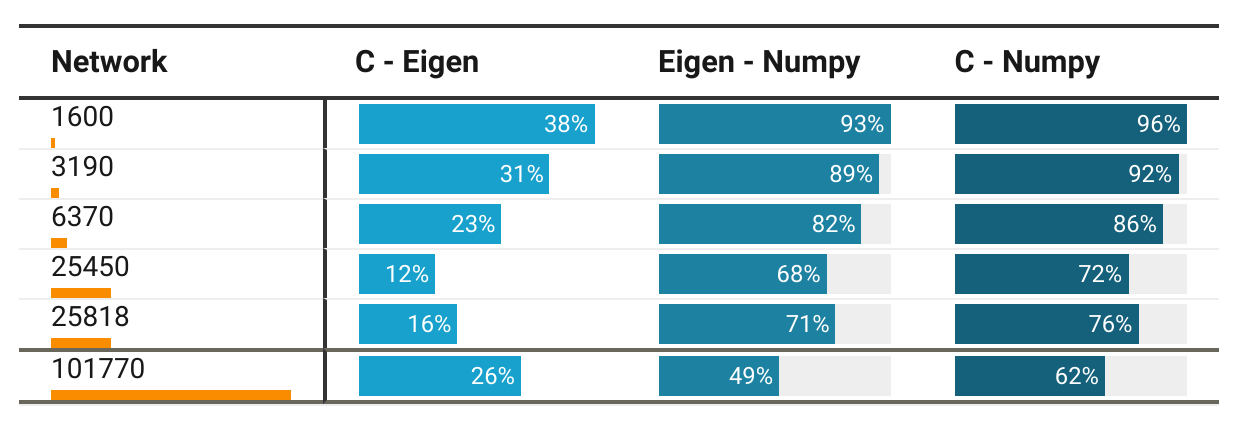
\includegraphics[scale=0.40]{exec_time_comparisons}
	\caption[Execution Time vs Model Parameters]{Percentage difference between the implementations. Example: C is 38\% faster than Eigen for the network size of 1600.}
\end{figure}

\begin{figure}[ht]
	\centering
	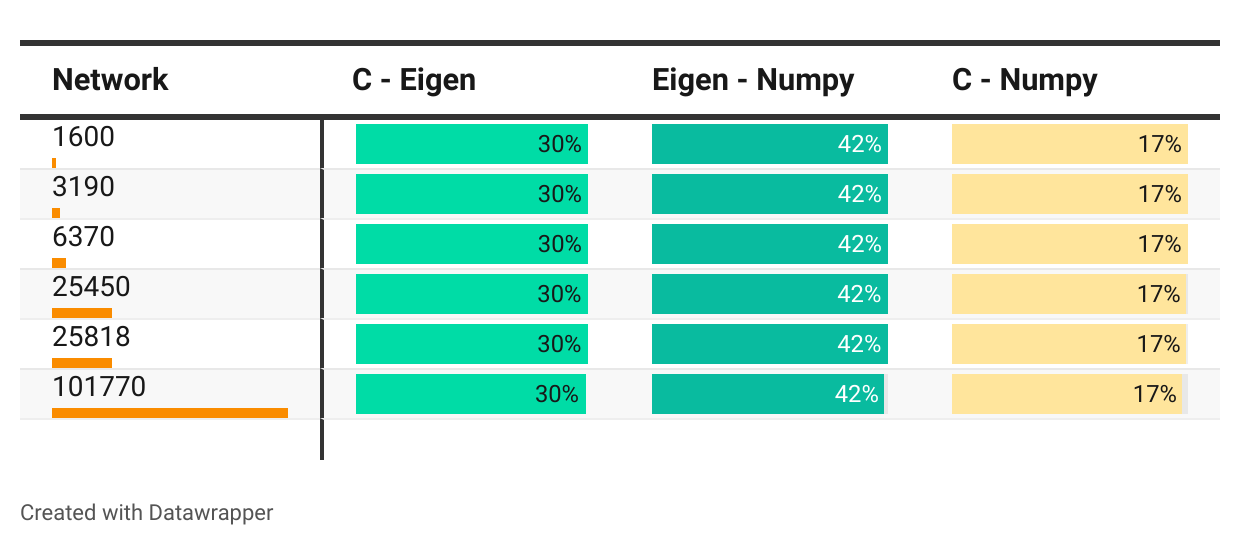
\includegraphics[scale=0.30]{peak_memory_comparisons}
	\caption[Peak Memory Utilisation]{Percentage difference between the implementations}
\end{figure}

The tables in (figure 6.4 and figure 6.5) shows the comparison between C-Eigen, Eigen-Numpy and C-Numpy. It is calculated as the percentage of 1 - (x/y) where x is performance value of the application which has lower value and y is performance value of the application that has higher number.

\subsection{C vs Eigen}
For smaller models, it can be observed that \texttt{C} is faster than Eigen (for the network size of 1600, \texttt{C} is 38 percent faster than Eigen). But as model becomes complex, Eigen perform better and the difference is execution time is less than 15 percent. Again the abnormal behaviour can be observed in case of network size 101770 where \texttt{C} is 26 percent faster than Eigen. More test on the \texttt{C} implementation needs to conducted to identify the bug causing this behaviour.

With regards to memory utilisation Eigen perform better than \texttt{C} by 30\%.

\subsection{C vs Numpy}
\texttt{C} constantly performs much better than Numpy. For the network size 101770, \texttt{C} is 62\% faster.
Numpy utilises 17\% more runtime memory than C.

\subsection{Eigen vs Numpy}
Similar to \texttt{C}, irrespective of network size, Eigen is faster than Numpy by similar margins.

Eigen is efficient in memory utilisation and 42\% better than Numpy.

% \subsection{Profiling}
% (TODO: perform profiling of the benchmark applications and note the results)

% \subsection{Failure/Fault testing}
% (TODO: perform the failure tests such as increases the network size until the application fails or system hangs.)

\section{Repurposing Scania ECU}
Scania ECU is like a black box with no information. A custom encased hardware that supports ethernet over modem and an UART interface along with hardware circuit schematic document was the only information available regarding the ECU. There is no information regarding the processor,  memory support, bootloader. As the ECU is a production unit, there is no development tools on device and no support to port packages and application to the ECU. Many features on the bootloader, kernel were disabled making it futile to execute the common commands that provide system information.

The task of repurposing the Scania ECU comprised of reverse engineering and obtaining the required hardware/software information and flashing a custom operating system to benchmark the neural network applications. The first task was partially successfully as hardware information such as processor, architecture, I/O interfaces, device tree and software information such as kernel, compiler, glic and versions was obtained. But information regarding the memory layout and boot flow could not be concretely reverse engineered. The second task was not achieved as flashing custom embedded linux always resulted in the ECU being bricked. Experiments conducted from booting the normal operation and from serial download mode had different issues and failed. While flashing from the normal boot, only the bootloader is replaced in the mtd partition. This could have failed because of incorrect u-boot image with wrong device trees or loading kernel failed as version mismatch between bootloader and kernel or checksum failure or size of the file is big overwriting a different region with crucial data. Serial download mode flashing required some crucial information regarding the memory load address and entry point for bootloader, kernel, root file system which is configured in the custom device tree. This information could be obtained from reverse engineering.

% ============================================
%        Discussion
% ============================================

\chapter{Discussion}

This chapter contains discussions on the experience while working on the project with the first section examining the process of developing the benchmark applications. The last section describes in brief the distribution of work on the project between the two authors.

\section{Developer Experience}

Embedded environments are greatly varied and working on these platforms are different compared to the more general platforms with comparably reduced support. The greatest challenge in writing the benchmark applications were in sourcing the binaries for the general purpose neural network frameworks. Both Tensorflow and PyTorch do not target the ARMv7 environment that was the primary target for this project. Finally the PyTorch source code was successfully compiled for our target environment using QEMU user-mode emulation.

\subsection{Reverse Engineering Scania C300}

\hyperref[rtc-c300]{Appendix II} contains a summary of the efforts involved in reverse engineering the C300 hardware. The project focus shifted to the iMX6SDB board after having spend considerable time on the C300.

\section{General Distribution of Work}

The reverse engineering efforts were done in unision between the authors by suggesting then attempting different ideas. The programming of the benchmark applications was completed by Prasanth Thomas Shaji while the testing and analysis of these applications on the were completed by Deepak Venkataram. The primary responsibilities of most activities were divided between the authors however they were performed in unison were possible. The benchmark applications and the report were version controlled in two seperate repositories containing commits from both authors.

\chapter{Conclusion and Future Work}

Developing neural network implementations for the embedded environment remains a challenging task. There are several challenges in the way for developing a machine learning framework for embedded devices that supports the fragmented embedded ecosystem. PyTorch had considerably higher performance than expected.


\section{Future Work}

Repurposing the Scania ECU is a technical challenge that was left incomplete during the project. The experience as detailed in \hyperref[rtc-c300]{Appendix II} and through out the report concluded without having ported the embedded linux onto the board.
